%! TEX root=./master.tex

\lecture{14}{Week 7}{Code Vulnerabilities}

\subsubsection{Worms And Viruses}
Both viruses and worms are designed to spread among computers, network and drives. Though they are fundamentally different:

\begin{description}
    \item[Worm:] is a program than runs by itself and which is capable to propagate a fully working version of itself to other computers.
    \item[Virus:] is code which adds itself to other programs ant it cannot run without its \textit{host} program.
\end{description}

In the early days of computers, worms were actually used in distributes systems for e.g. update purpose. The first \textit{malicious} worms was written in 1988 by Robert Morris and was designed to count the number of hosts on a network. 

\subsubsection{Stack Overflow Bugs}
This is one of the simplest code vulnerability bugs one can exploit.

\code{gets} is a C functions which ready input till it receives an \textit{end-of-file} character and stores them in an array designated by a pointer. The problem with this early implementation was, that there is no way to specify the maximal number of characters to read.

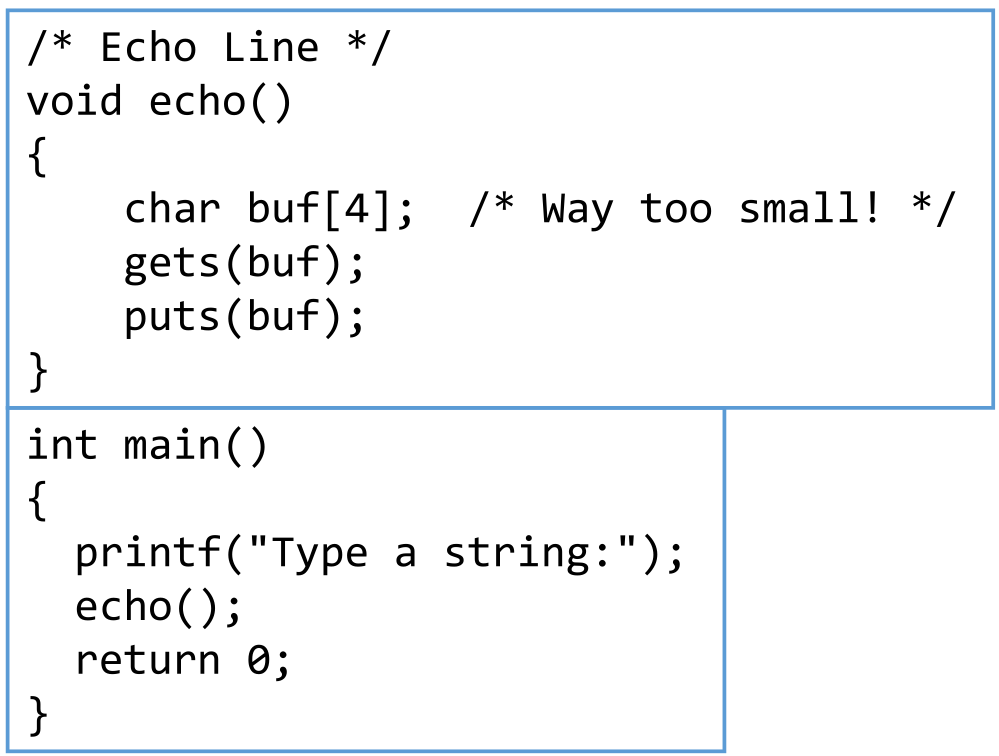
\includegraphics[width=0.8\textwidth]{14_gets.png}

The previous code works perfectly for inputs of length $3$ (the $4$-th byte is required for the end character) or maybe even for a few more bytes, but when we input a large amount of characters we get a segmentation fault. 

A stack frame of a certain size gets initialized and the buf variable is stored within in.

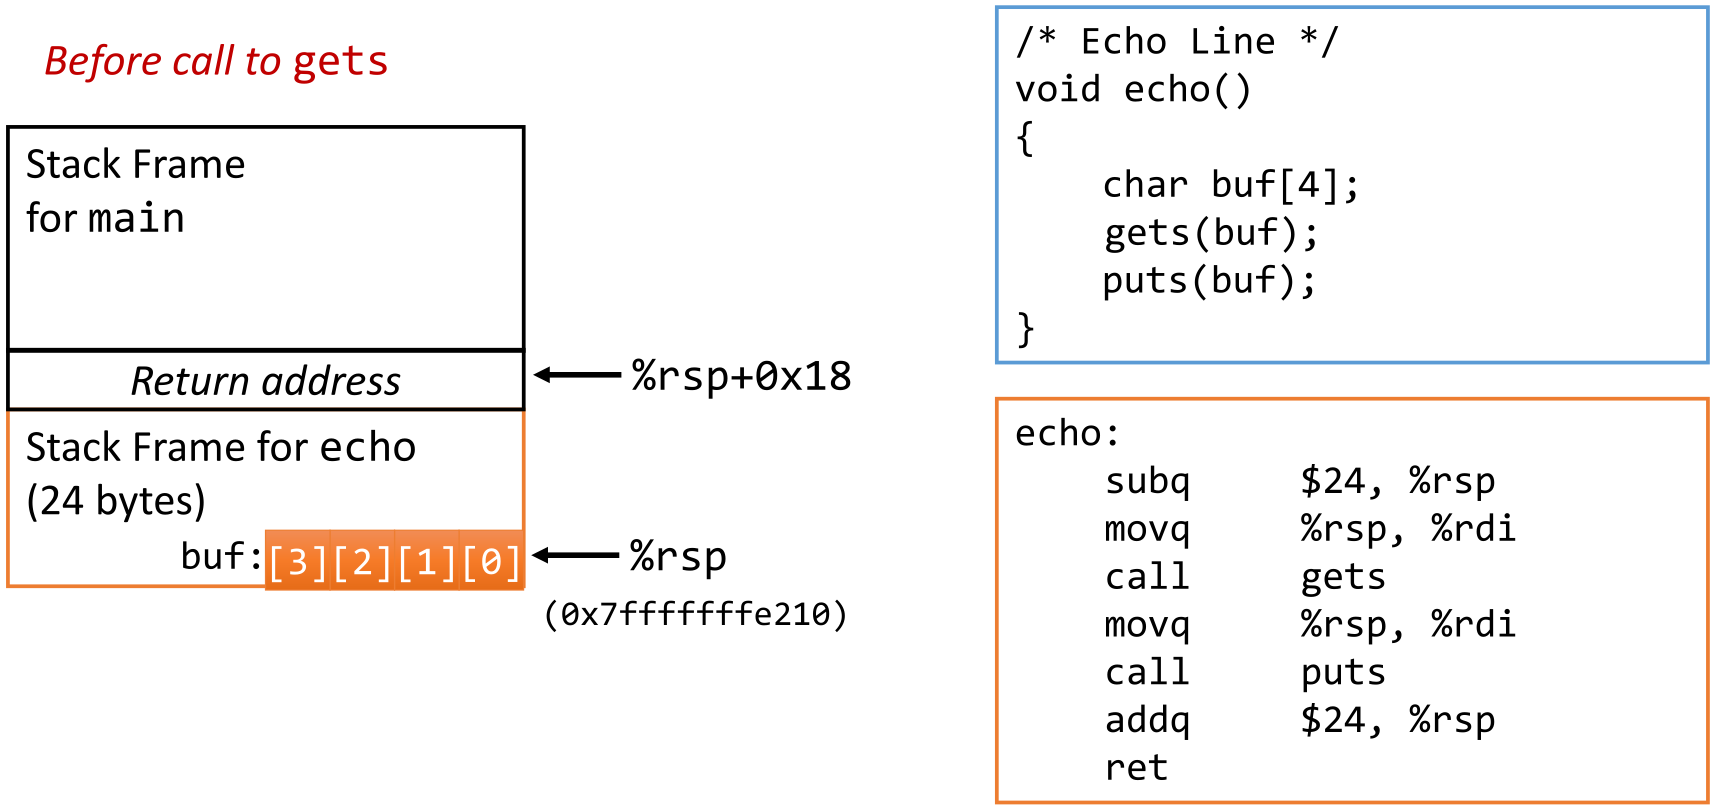
\includegraphics[width=0.8\textwidth]{14_getsStack.png}

As long as we only overwrite data in the stack frame, this may not cause direct problems, when when the return address gets overwritten, we will receive a segmentation fault.

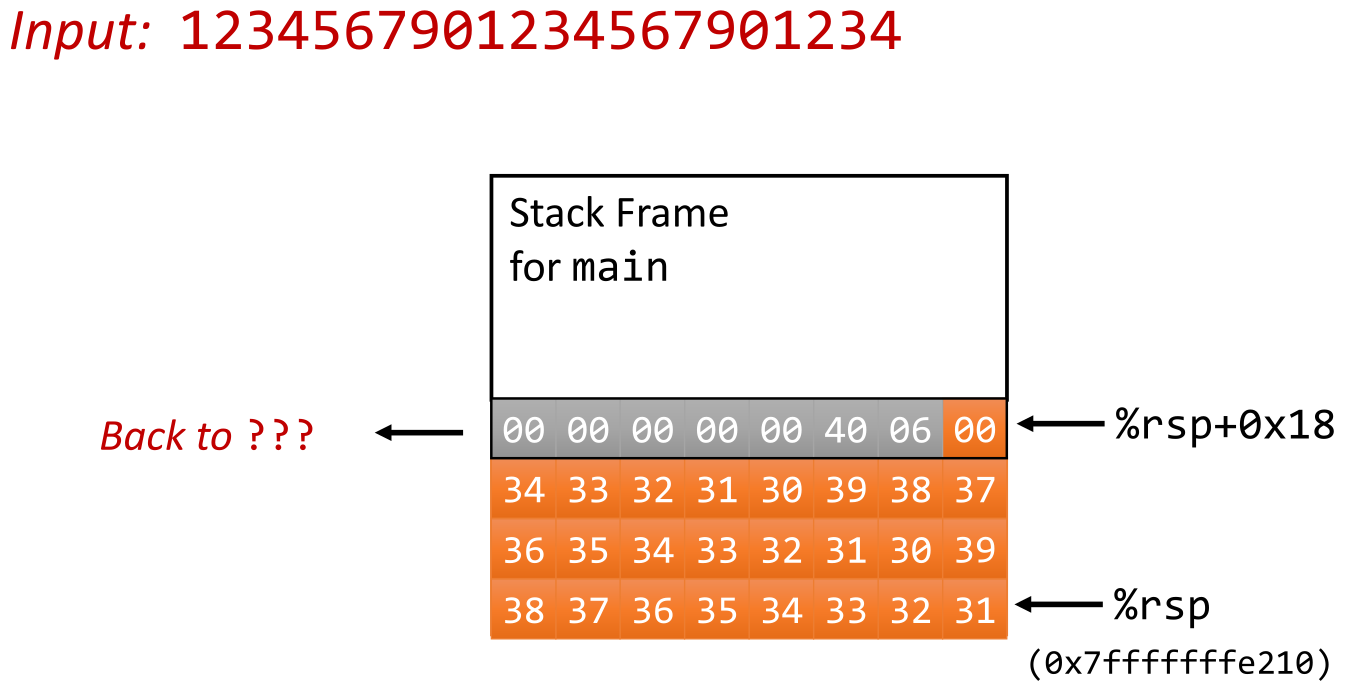
\includegraphics[width=0.8\textwidth]{14_getssegmentation.png}

Instead of simply crashing the program, we may make malicious use of this vulnerability. My overwriting the return address of another stack frame and make it point to some exploit code which we have pushed to the stack via gets.

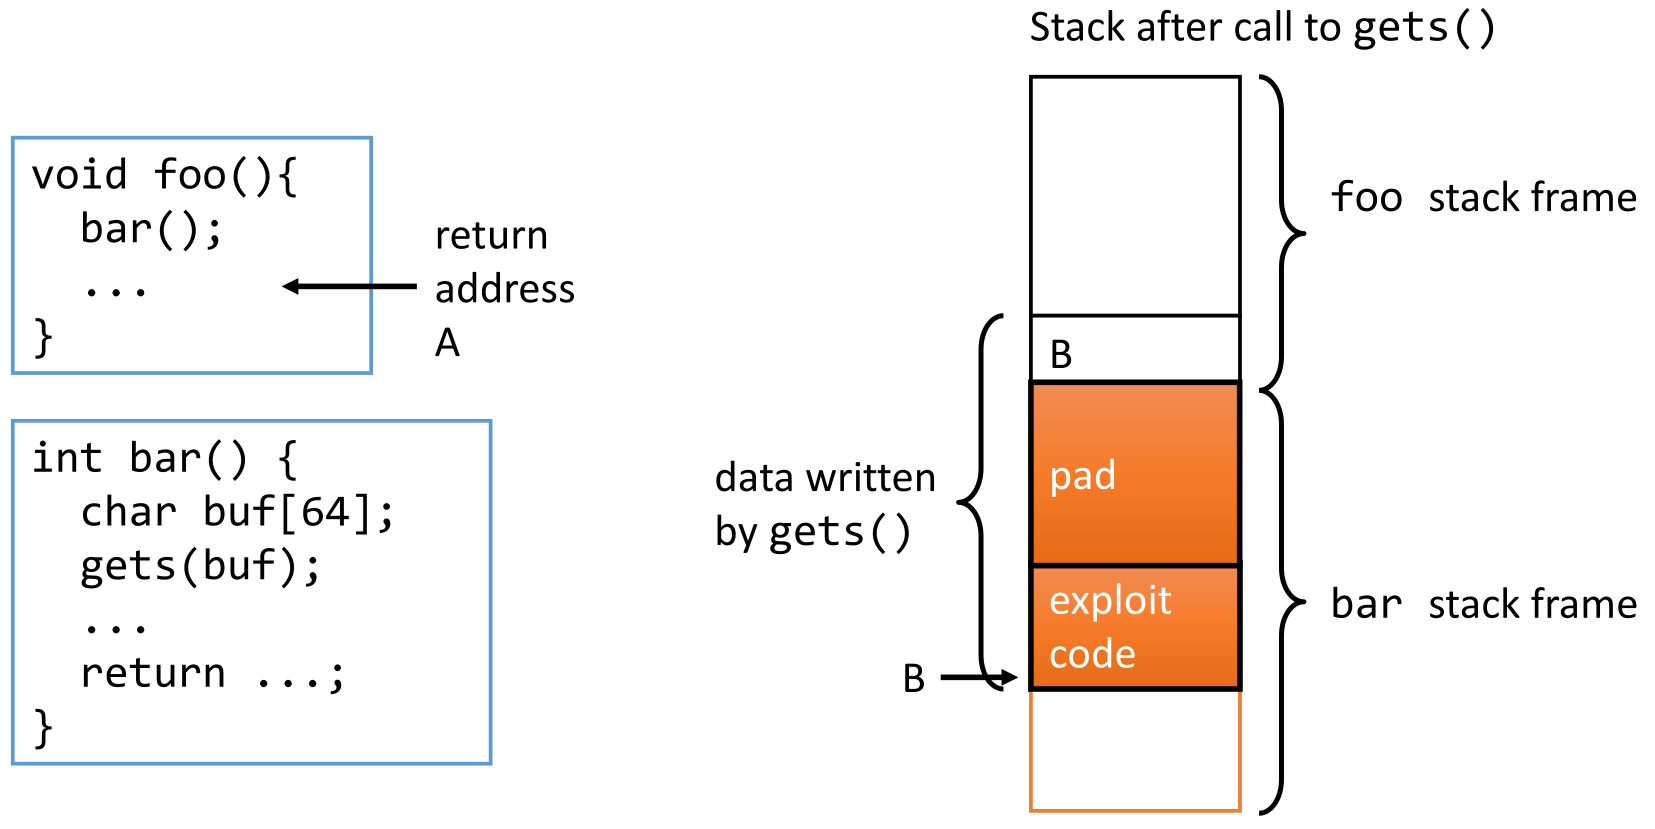
\includegraphics[width=0.8\textwidth]{14_maliciousoverflow.png}

There used to be a server called \code{fingered} which used \code{gets}. Instead of calling it like \code{finger username@addres}, one could execute something like \code{finger "exploit code padding new-return-address"} which then gets executed on the root shell.

\paragraph{Prevent Stack Overflow Issues}
There are several ways to prevent these issues. One should for example always use the more modern and robust functions. I.e. use \code{fgets} instead of \code{gets}, \code{strncpy} instead of \code{strcpy} and \code{fgets} instead of \code{scanf} for reading strings (or use \code{\%ns} instead if \code{\%s}).

Further, one should also always take care when defining these limits. It is actually really hard to get them right. It can easily happen that the end character is forgotten.

Compilers do have a notion about libraries (which is not only something positive...) and may detect such issues. For experimentation purpose we can disable this feature using the flags \code{-D\_FORTIFY\_SOURCE=0} and \code{-fno-stack-protector}.

In order to make it more difficult for a attacker to guess the right address, stack offsets are initialized at random. Furthermore, some CPUs can make certain parts of the memory read- or write only. Or they can make the stack non-executable, meaning that no code on the stack can be executed. However, we can still use e.g. the heap for exploit code and therefore, this is not really a fix.

All in all, even though this problem is mostly  fixed, it still pops up from time to time. 

\subsection*{Floaging Point}
\subsubsection{Representing Floating-Point Numbers}
Fractional binary numbers can be very intuitively represented as $\sum_{k=-j}^{i} b_k \cdot 2^k$. All bits to the right of some \textit{binary point} represent fractions of powers of $2$.

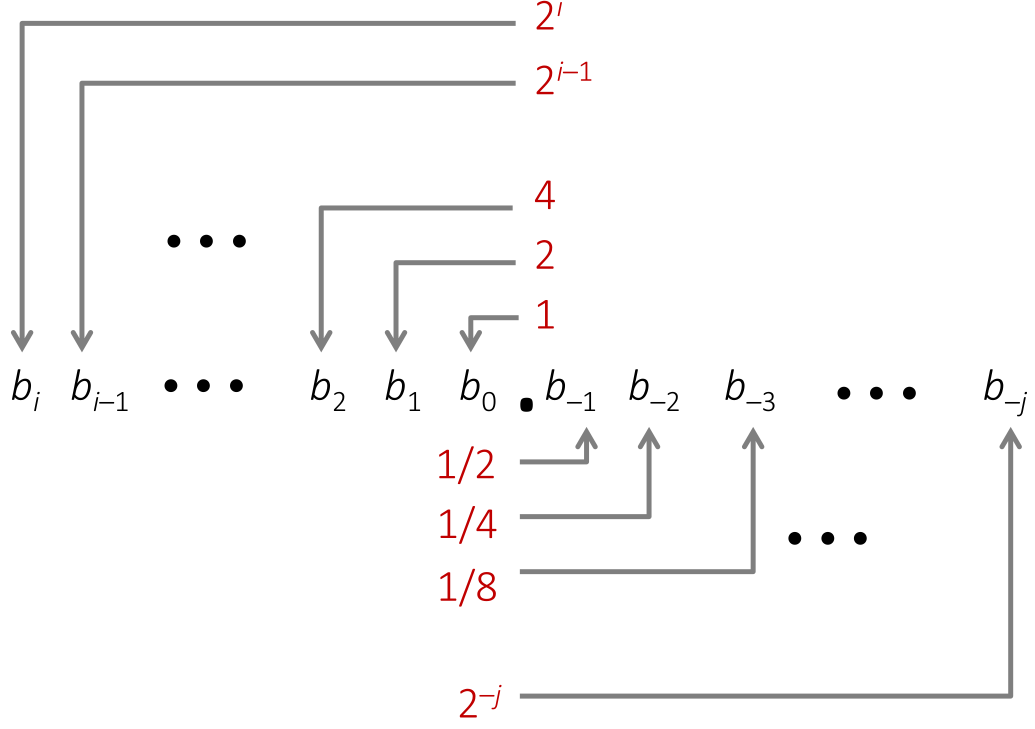
\includegraphics[width=0.8\textwidth]{14_fractionalrepresentation.png}

As we are used to from integers, a right shift represents a division of $2$ and a left shift a multiplication by $2$. 

The problem with this representation is that, we can only exactly represent numbers which are of the form $\frac{x}{2^k}$. In order to represent any number exactly we would need infinitely many decimal points.

\paragraph{IEEE Floating Point}
In the early days, there was no standard on how to represent binary numbers, and all CPU manufactures implemented their own format. In 1985 the first standard for floating point arithmetic was introduced. It was supported by all major CPUs.

Floating point numbers are represented in the form $(-1)^S \cdot M \cdot 2^E$.
\begin{description}
    \item[S:] sign bit determines whether the number is positive or negative.
    \item[M:] is the significant and it is a fractional value in the range $)1.0, 2.0)$.
    \item[E:] exponent weight.
\end{description}

The $M$ and $E$ are not directly stored as twos complement, but encoded in a specific was. This allows the format to represent a much wider range. The encoding is as follows:
\begin{description}
    \item[s:] directly represents the $S$ and is the MSB of the encoding.
    \item[exp:] is the encoding of $E$
    \item[frac:] is the encoding of $M$
\end{description}

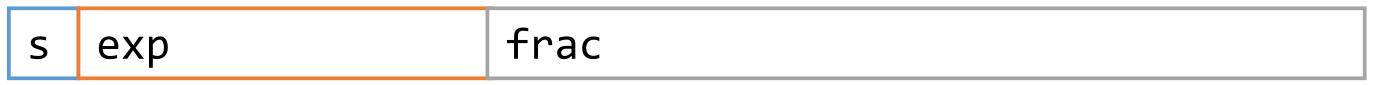
\includegraphics[width=0.8\textwidth]{14_encoding.png}

The length of the exp and frac section is determined by the used Standard.

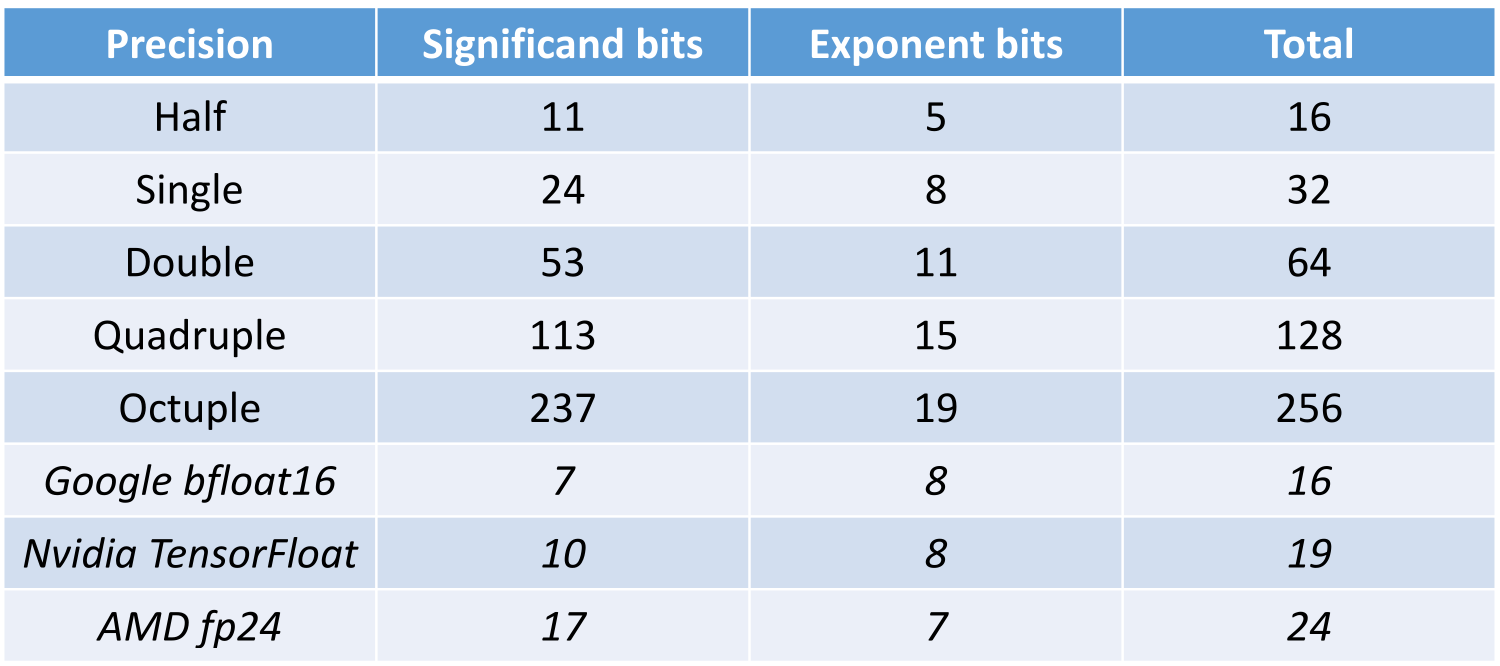
\includegraphics[width=0.8\textwidth]{14_percisionstandardtable.png}

There used to be the two single and double precision standards. Over time the total length got bigger. But only recently a few other, much shorter non-standards, but widely used ones, were introduced. They are used mainly for machine learning. One found out that it is worth trading precision for efficiently.

\paragraph{Floating Point in C}
In C99, float (single precision) and double (double precision) are guaranteed to have a certain size independent of the machine. Other types vary in length.

When casting one type to another, the bit representation changes. This is very different from the signed/unsigned integer representation, where only the interpretation changed.
\begin{description}
    \item[double/float $\to$ int:] truncates fractional parts which is equivalent to a rounding towards zero. The behaviour is undefined when out of range.
    \item[int $\to$ double:] As long as the int has less that $\le 53$ bit word size, the conversation is exact.
    \item[int $\to$ float:] Will round according to the rounding mode.
\end{description}

Floating point numbers are einher normalized, or denormalized:
\paragraph{Normalized Values}

\begin{itemize}
    \item This are numbers, where $exp \neq 000 \dots 0$ and exp $\neq 111 \dots 1$.
    \item E is encoded as $E = Exp - Bias$ 
        \begin{description}
            \item[Exp:] is the unsigned value of exp
            \item[Bias:] is equal $2^{e-1} - 1$, where $e$ is the number of exponent bits.
                \begin{description}
                    \item[Singe Percision:] $Bias = 127, Exp \in [1, 254], E \in [-126, 127]$
                    \item[Double Perc.:] $Bias = 1023, Exp \in [1, 2046], E \in [-1022, 1023]$
                \end{description}
        \end{description}
    \item M is equal to $1.xxx \dots x_2$ where $xxx \dots x$ are the bits of frac.
        \begin{itemize}
            \item Minimum when $000 \dots 0 \implies M = 1.0$
            \item Maximum when $111 \dots 1 \implies M = 2.0 - \epsilon$
        \end{itemize}
\end{itemize}

\paragraph{Example}
Normalized encoding of $15213.0$:

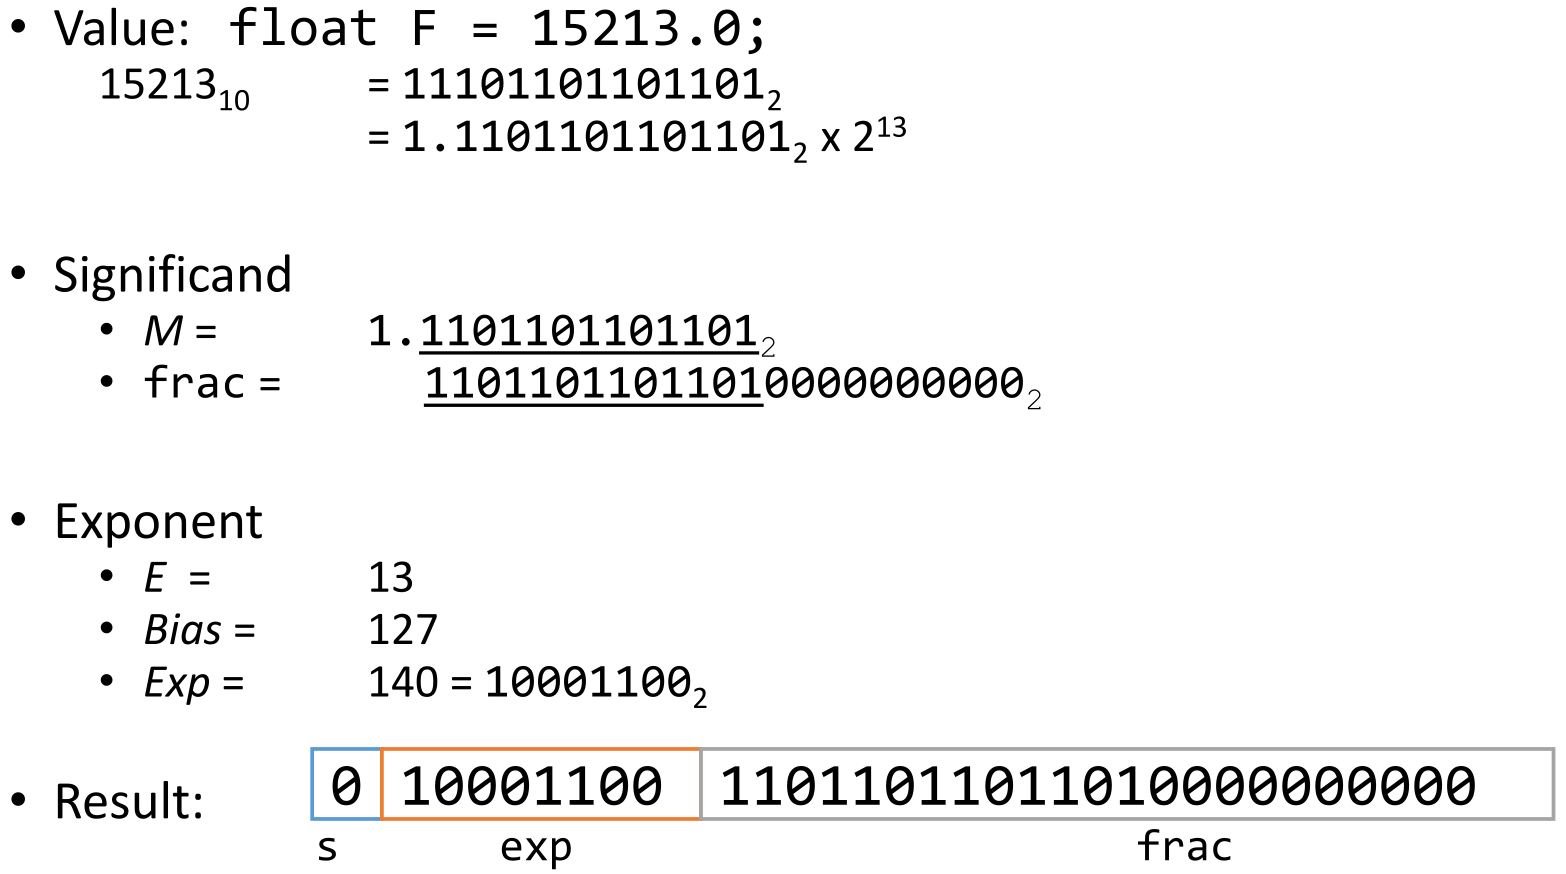
\includegraphics[width=0.8\textwidth]{14_normalizedexample.png}

\paragraph{Denormalized Values}
\begin{itemize}
    \item These are numbers, where $exp = 000 \dots 0$.
    \item E is encoded as $E= -Bias + 1$
        \begin{description}
            \item[Bias:] is equal $2^{e-1} - 1$, where $e$ is the number of exponent bits.
                \begin{description}
                    \item[Singe Percision:] $Bias = 127, Exp \in [1, 254], E \in [-126, 127]$
                    \item[Double Perc.:] $Bias = 1023, Exp \in [1, 2046], E \in [-1022, 1023]$
                \end{description}
        \end{description}
    \item M is equal to $0.xxx \dots x_2$ where $xxx \dots x$ are the bits of frac.
\end{itemize}

When $exp = 000 \dots 0$ and one if $frac = 000 \dots 0$, the number is zero. Depending on $s$, we have actually $-0$ and $+0$. This is actually useful to distinguish between convergence from below and from above.

When $exp = 000 \dots 0$ and $frac \neq 000 \dots 0$ we represent numbers very close to $0.0$. Such numbers are \textit{equispaced}. Also we notice, that we lose precision the smaller the number gets.

\paragraph{Interesting Numbers}
This table show some interesting floating point numbers.

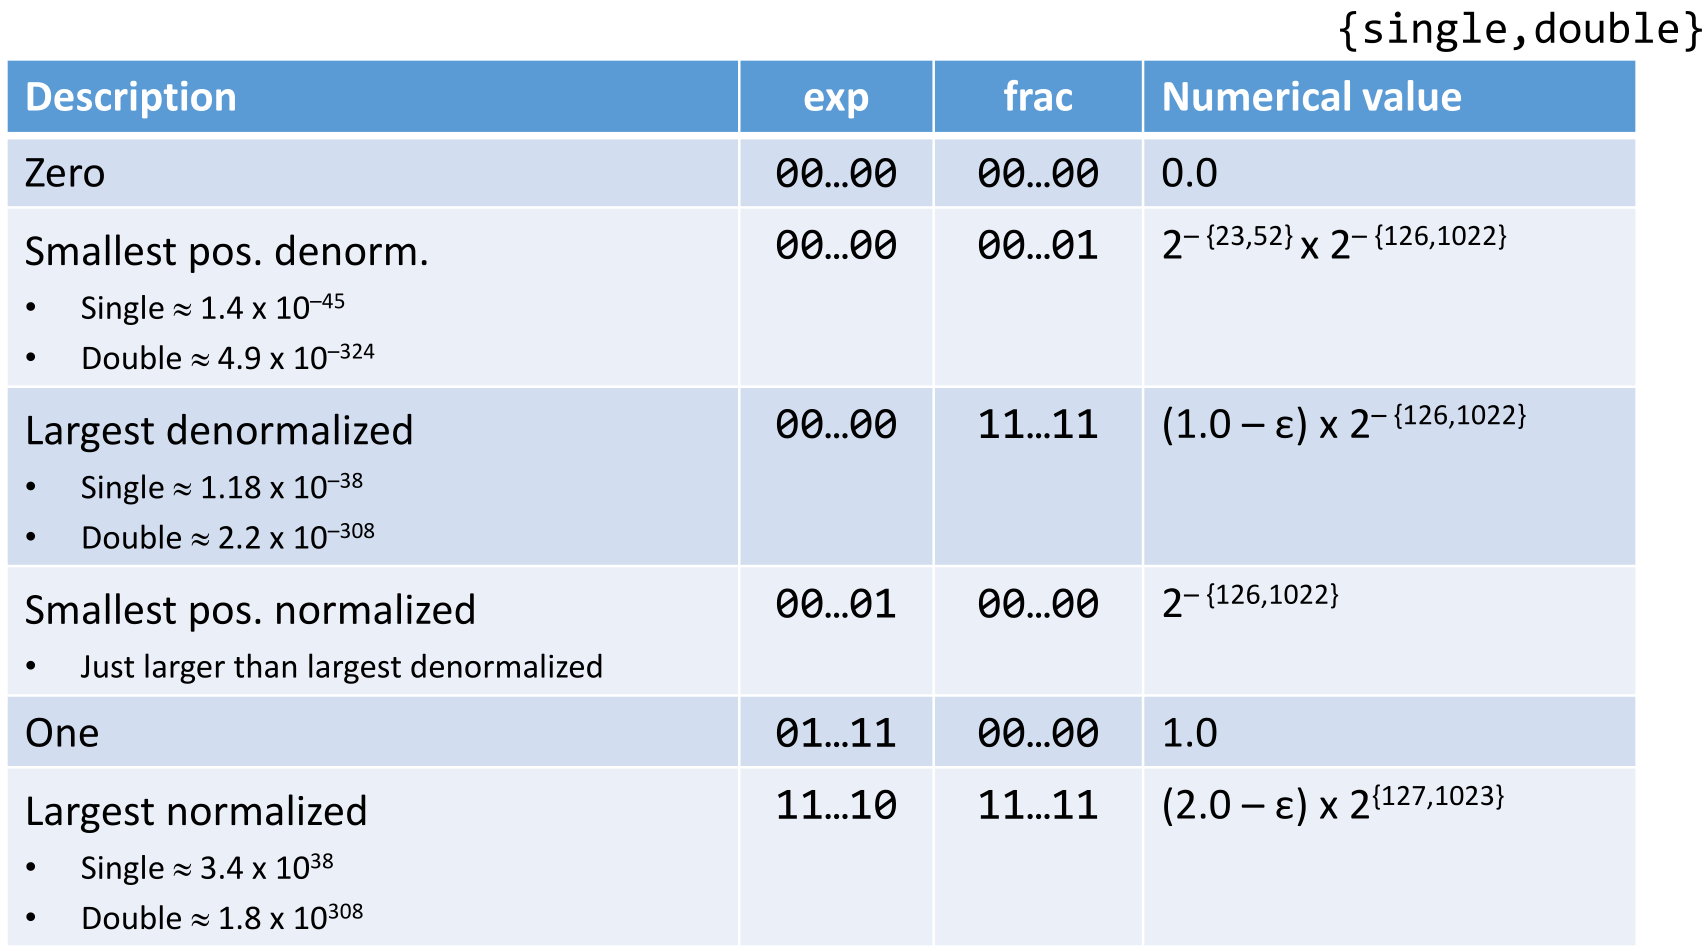
\includegraphics[width=1\textwidth]{14_interstingnumbers.png}

\paragraph{Special Values}
The description above does not handle the case when $exp = 111 \dots 1$. This value is used as follows:
\begin{description}
    \item[$\mathbf{exp = 111 \dots 1, frac = 000 \dots 0}$:] Represents $+\infty$ and $-\infty$ as well as operation overflow.
        \item[$\mathbf{exp = 111 \dots 1, frac \neq 000 \dots 0}$:] Represents NaN, i.e. cases where no numerical value can be determined.
\end{description}

\paragraph{Spacial Properties}
\begin{itemize}
    \item The floating point $+0$ is zero for all bits. This is equivalent for the integer zero.
    \item The allow comparison with unsigned integer with the cravats:
        \begin{itemize}
            \item Compare sign bits
            \item Consider $-0 = 0$
            \item Nan is problematic since what should the comparison yield?
        \end{itemize}
\end{itemize}

\subsubsection{Floating-Point Ranges}
For a $8$-bit floating point representation with $1$ bit for s, $4$ bits for exp and $3$ bits for frac

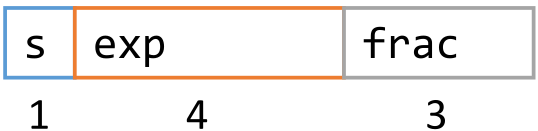
\includegraphics[width=0.8\textwidth]{14_tinyfloat.png}

this table shows the positive range of our $8$-bit number

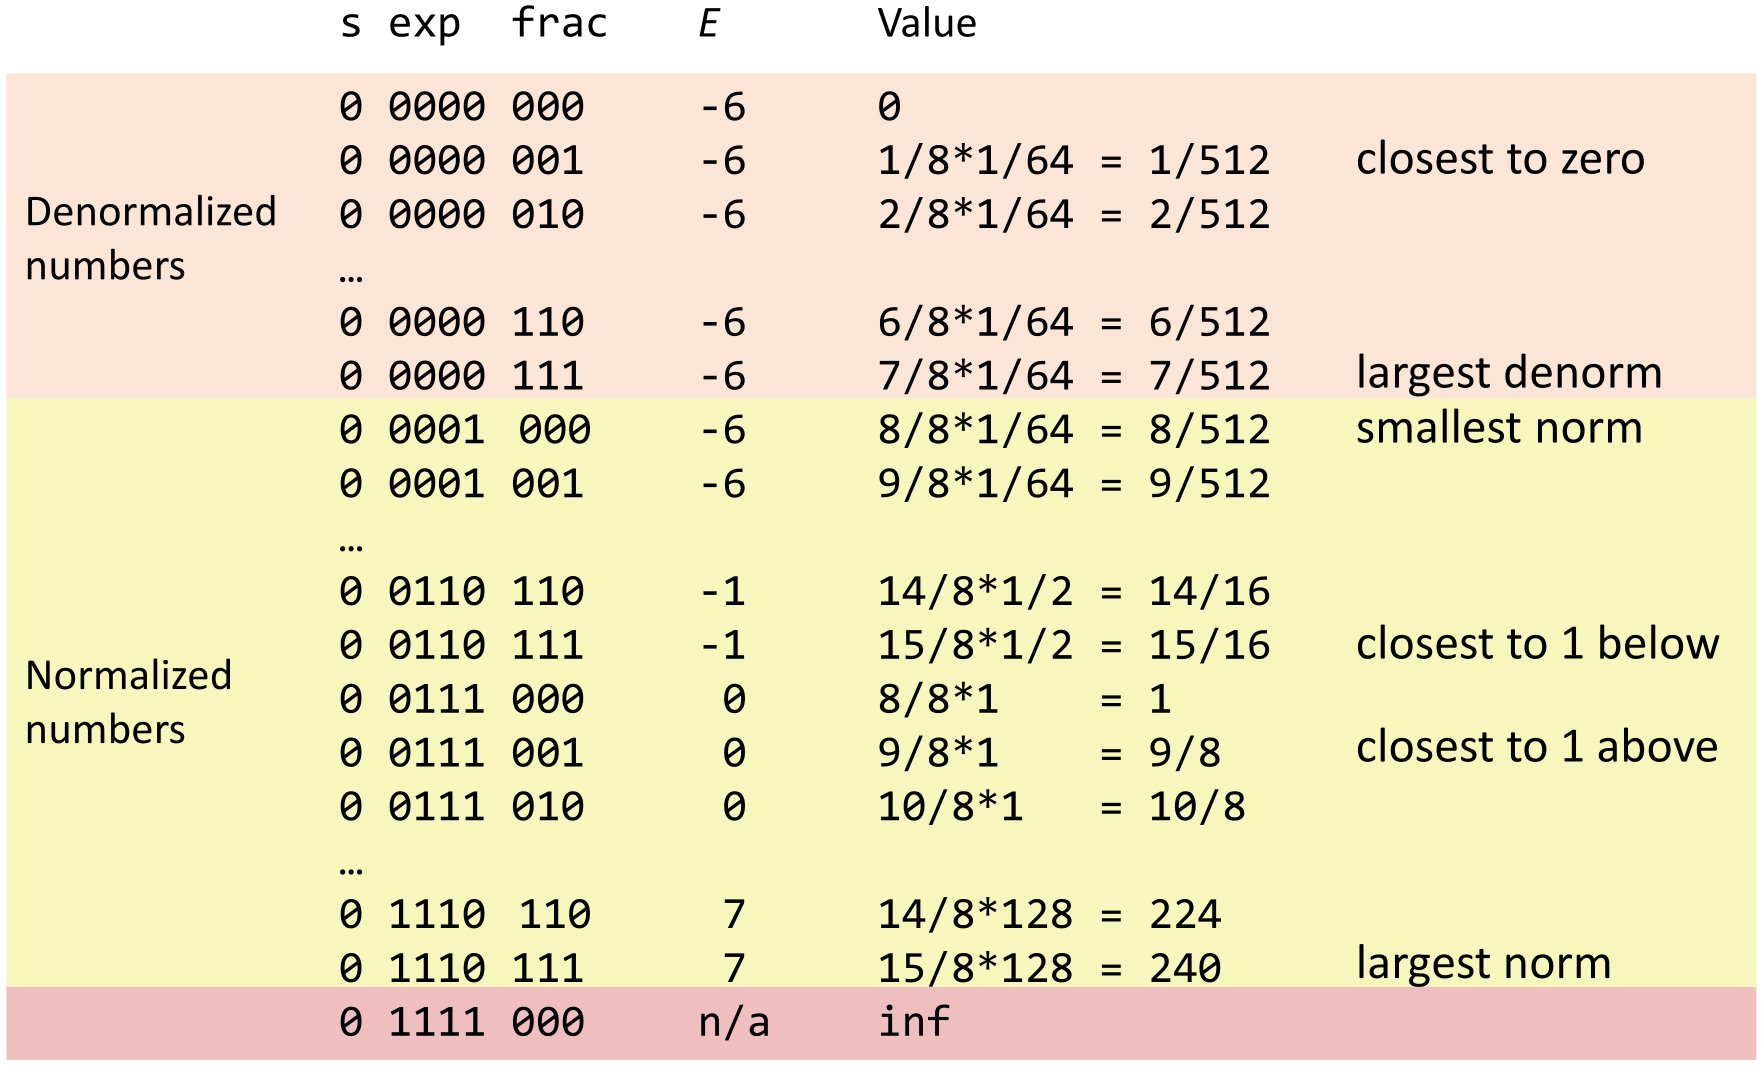
\includegraphics[width=1\textwidth]{14_tinytable.png}

For a $6$-bit floating point representation with $1$ bit for s, $3$ bits for exp and $2$ bits for frac

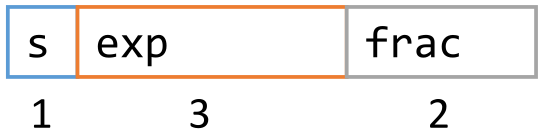
\includegraphics[width=0.8\textwidth]{14_6bitfp.png}

We can see that the distribution gets denser towards zero

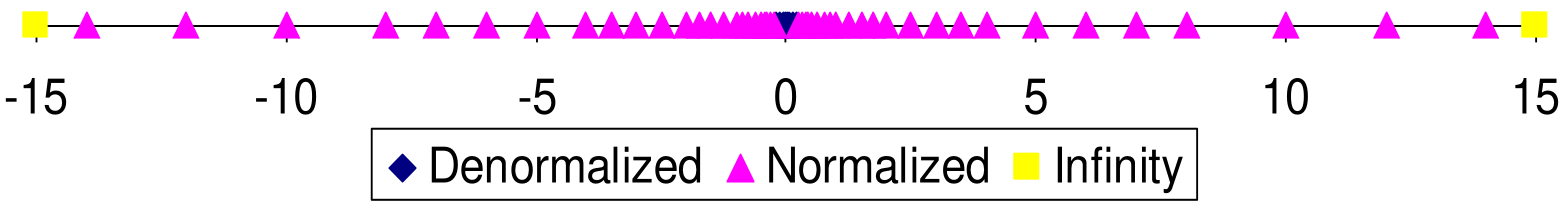
\includegraphics[width=1\textwidth]{14_6bitoverview.png}

When zooming in, we can see the equispaced denormalized values

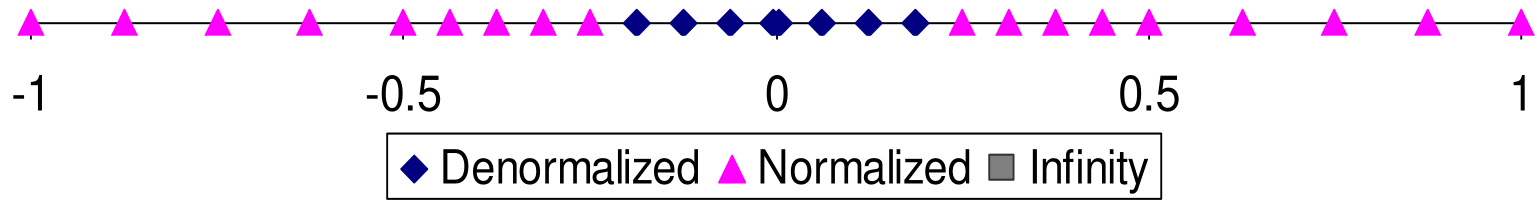
\includegraphics[width=1\textwidth]{14_6bitzoomin.png}

